\begin{frame} \frametitle{\vspace*{0.5cm}Results: Vorticity dynamics for the 10 MPa trapezoidal wave}
  \begin{figure}
    \centering
    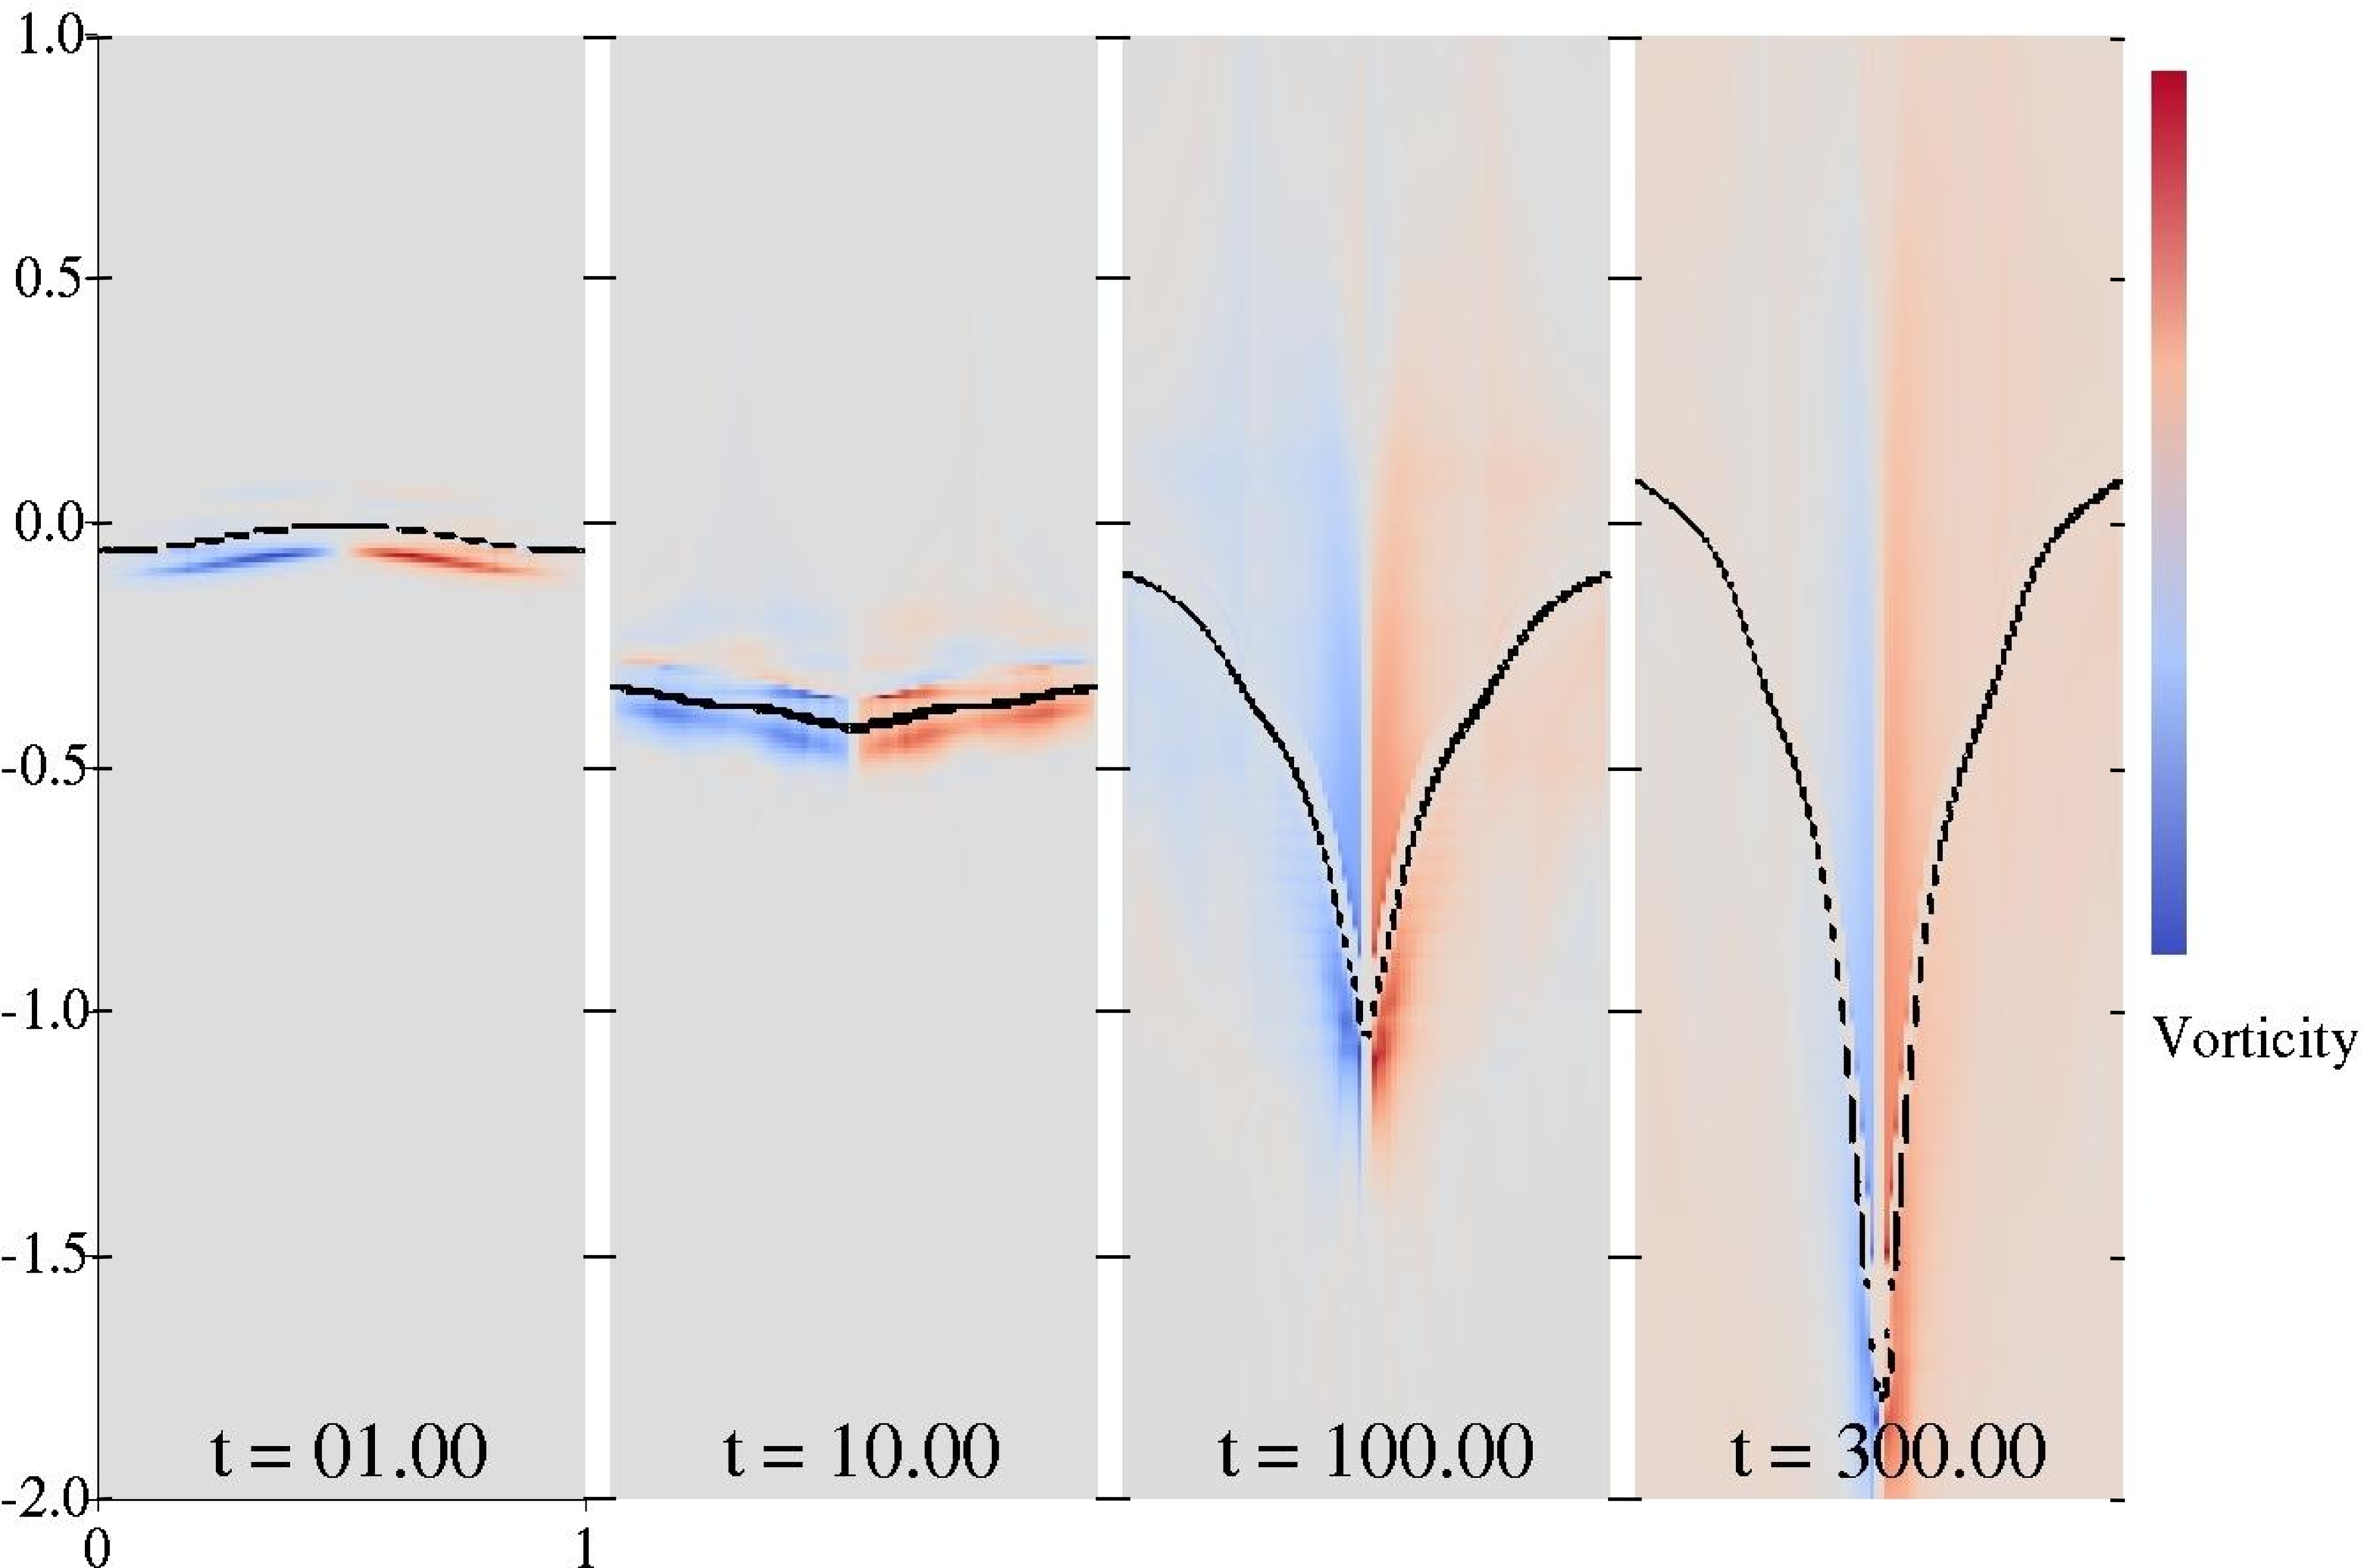
\includegraphics[width=0.8\textwidth]{../figs/lung_figs/snapshots_vorticity_t1}
  \end{figure}
  % 
  {\small
    \begin{itemize}
    \item Vorticity initially deposits in air-dominated $(y_0<0.5)$
      fluid of the interface.
    \item As the interface evolves, some vorticity advects with it.
    \end{itemize}
  }
  \note{
    \begin{itemize}
    \item A linear scale that changes each timestep is used for visual
      reasons.
    \item Air-domination is surprising because almost all of the wave
      is reflected so most of energy of the fluid stays in the water
      because of the high impedance mismatch.
    \end{itemize}
  }
\end{frame}
%%% Local Variables:
%%% mode: latex
%%% TeX-master: "../main"
%%% End:
